\section{Lecture 25.00: F Test}
\begin{figure}[!htbp]
    \centering
    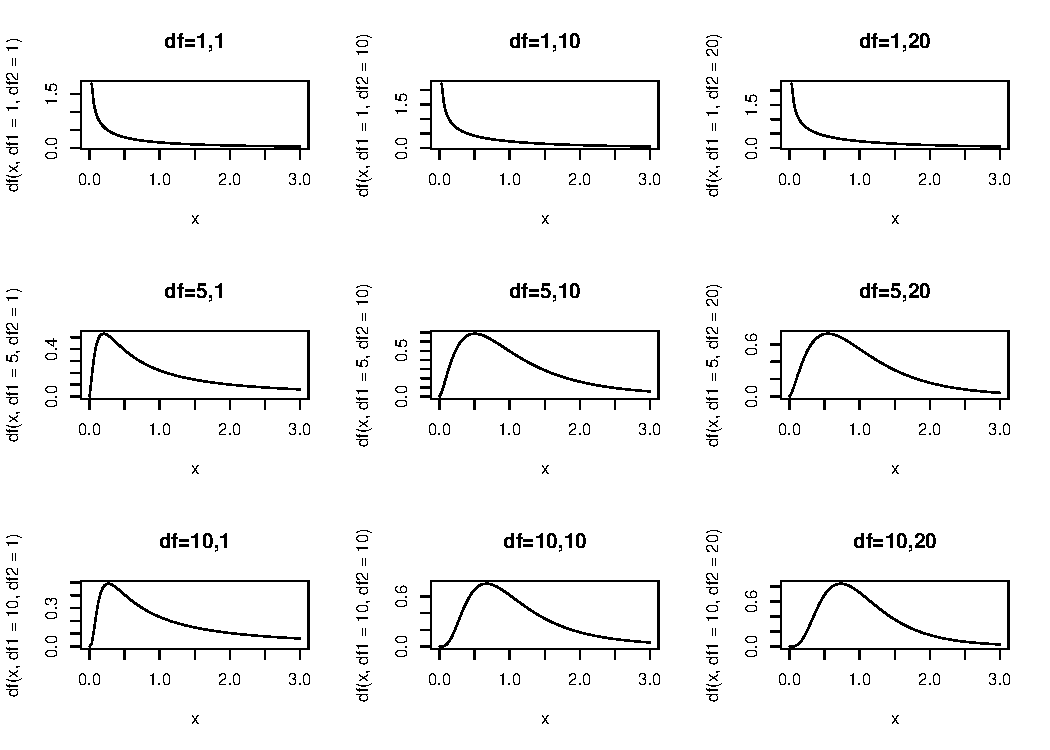
\includegraphics[width=0.7\textwidth]{fdistn.pdf}
    \caption{$ F $ distribution}
\end{figure}
\begin{Theorem}{}{}
    Let $ X \sim \chi^2(m) $ and $ Y \sim \chi^2(n) $, then
    \[ \frac{X/m}{Y/n} \sim F(m,n) \]
\end{Theorem}
\begin{Theorem}{}{}
    Let $ X \sim F(m,n) $ and $ Y \sim 1/X $, then
    \[ Y \sim F(n,m) \]
\end{Theorem}
\begin{Example}{}{}
    $ \alpha=\Prob{F(20,4)>4}=(0.05,0.1) $ since
    \begin{center}
        \begin{NiceTabular}{c|ccc}
            $\alpha$       & 0.1  & 0.05 & 0.01 \\
            \midrule
            critical value & 3.84 & 5.80 & 14.0
        \end{NiceTabular}
    \end{center}
    In R, we can directly calculate $ \alpha $ with \code{1-pf(4,20,4)=0.094}.
\end{Example}
\[ \tilde{F}=\frac{\widetilde{\MS{Trt}}}{\widetilde{\MS{Res}}}  \]
Now, $ \widetilde{\MS{Res}}=\tilde{\sigma}^2 $. We know
\begin{equation}\label{eq:1}
    \frac{\tilde{\sigma}^2\text{df}_\text{Res}}{\sigma^2} \sim \chi^2(\text{df}_{\text{Res}})
\end{equation}
Similarly,
\begin{equation}\label{eq:2}
    \frac{\widetilde{\MS{Trt}}\text{df}_\text{Trt}}{\sigma^2} \sim \chi^2(\text{df}_\text{Trt})
\end{equation}
Divide~\ref{eq:2} by~\ref{eq:1} to get
\[ \frac{\widetilde{\MS{Trt}}}{\widetilde{\MS{Res}}} \sim F(n,d) \]
where $ n=\text{df}_\text{Trt} $ and $ d=\text{df}_\text{Res} $.

\subsection*{When is $ F $ large?}
\[ \E{\tilde{F}}=
    \E*{\frac{\widetilde{\MS{Trt}}}{\widetilde{\MS{Res}}}}{\color{red}\approx}
    \frac{\E{\widetilde{\MS{Trt}}}}{\E{\widetilde{\MS{Res}}}}
    =\frac{\sigma^2+r \dfrac{\sum_{i=1}^t \tau_i^2}{t-1} }{\sigma^2}  \]
\[ \E{\tilde{F}}=1+\frac{r}{\sigma^2} \frac{\sum_{i=1}^t \tau_i^2 }{t-1}  \]
If $ \tau_1=\tau_2=\cdots=\tau_t=0 $, then $ \E{\tilde{F}}=1 $.
However, if even one $ \tau $ is not zero, then $ \E{\tilde{F}}>1 $.

\subsection*{$F$ Test}
\begin{enumerate}[(1)]
    \item $ H_0 $: $ \tau_1=\tau_2=\cdots=\tau_t=0 $ versus $ H_a $: at least one $\tau$ is not zero.
    \item $ \displaystyle d=\frac{\MS{Trt}}{\MS{Res}}  $ where $ D \sim F(\text{df}_\text{Trt},\text{df}_\text{Res}) $
    \item $ p\text{-value}=\Prob{D>d} $
    \item Conclusion.
\end{enumerate}
